\section{Аннотация}
\textbf{Цель работы:} исследование спектра колебаний электрических сигналов.\\

В данной работе проводится исследование спектров различной формы (последовательности прямоугольных импульсов и цугов, а также амплитудно-модулированных гармонических колебаний (АМ-сигналов)). Спектры этих сигналов наблюдаются с помощью спектроанализатора, входящего в состав USB-осциллографа. Проводится проверка нескольких теоретических соотношений.

\section{Теоретические сведения}

Рассмотрим функцию вида
\begin{equation*}\label{f}
	f(x) = \sum_{n=1}^{N}A_n \cos(\omega_n t -\alpha_n),
\end{equation*}
где $ A_n, \omega_n, \alpha_n $ -- постоянные величины. Множество пар $ (\omega_i, A_i) $ называется спектром $ f(x) $ и может быть конечным или бесконечным.

Периодический сигнал может быть представлен в виде ряда Фурье:
\begin{equation*}\label{key}
	f(t) = \frac{a_0}{2}+\sum_{n=1}^{\infty}(A_n \cos(n \Omega_1 t - \psi_n)),
\end{equation*}
где $ a_0/2 = const $ -- среднее значение функции, $ A_n $ -- амплитуды членов разложения. Спектр любой периодической функции можно представить в виде набора гармонических колебаний с дискретными частотами $ \Omega_1 = \frac{1}{T_1}, 2\Omega_1, \ldots $ и постоянной составляющей с нулевой частотой. Такой спектр называется линейчатым или дискретным.

Непериодический сигнал представим в виде интеграла Фурье. В данной работе исследование таких сигналов не проводится.

Для периодического прямоугольного сигнала $ \left< V \right> = V_0 \frac{\tau}{T} $, $ A_n \sim \frac{\sin x}{x} $. Здесь и далее шириной спектра $ \Delta \nu $ называем расстояние от главного максимума до 1-го нуля огибающей. При этом выполнено соотношение неопределённостей:
\begin{equation*}\label{eq:неопр}
	\Delta \nu \tau \simeq 1
\end{equation*}

\begin{figure}[h]
    \centering
    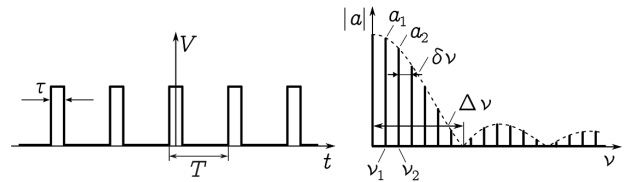
\includegraphics[width=15cm, height=4cm]{rectangle_signal.jpg}
    \caption{Периодическая последовательность импульсов и её спектр}
    \label{fig:table1}
\end{figure}

Для последовательности цугов с длительностью $ \tau  $ и периодом $ T $ разложение в спектр представлено на рис. 2:

\begin{figure}[h]
    \centering
    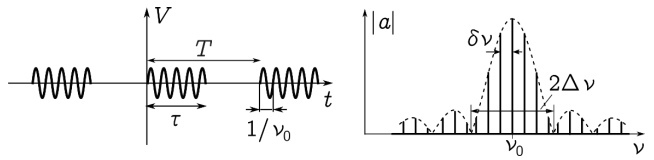
\includegraphics[width=15cm, height=4cm]{CUG.jpg}
    \caption{Периодическая последовательность цугов и её спектр}
    \label{fig:table1}
\end{figure}

В случае АМ-колебаний, сигнал определяется формулой:
\begin{equation*}\label{key}
	f(t) = A_0 \left(1+m \cos \Omega t \right) \cos \omega_0 t,
\end{equation*}
где $ m $ -- глубина модуляции.
Спектр такого сигнала на рис. 3. Причём амплитуды синусов $ \omega_0 \pm \Omega $ равны $ m/2 $, а все начальные фазы одинаковы. То есть,
\begin{equation*}\label{new}
	\frac{a_\text{бок}}{a_\text{осн}} = \frac{U_{min}^S}{U_{max}^S} = \frac{m}{2}
\end{equation*} Глубину модуляции можно рассчитать по формуле:
\begin{equation*}\label{m}
	m = \frac{A_{max}-A_{min}}{A_{max}+A_{min}}
\end{equation*}
\begin{figure}[h]
    \centering
    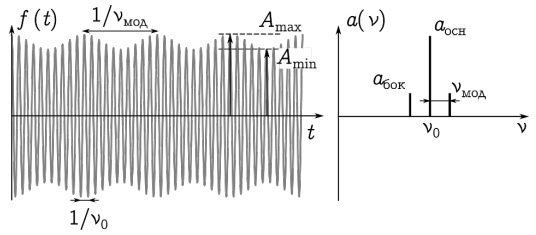
\includegraphics[width=12.5cm, height=5cm]{AM.jpg}
    \caption{Гармонический амплитудно-модулированный сигнал и его спектр}
    \label{fig:table1}
\end{figure}


\section{Оборудование и инструментальные погрешности}

\textbf{В работе используются:} генератор сигналов произвольной формы, цифровой осциллограф с функцией быстрого преобразования Фурье или цифровой USB-осциллограф, подключённый к персональному компьютеру.

Функциональный генератор позволяет сформировать два различных электрических сигнала, которые выводятся на два независимых канала USB-осциллографа.

Инструментальные погрешности считаются малыми.
